\lstdefinestyle{javaStyle}{
  language=Java,
  numbers=left,
  stepnumber=0,
  numbersep=10pt,
  tabsize=2,
  showspaces=false,
  showstringspaces=false
}

 \lstdefinestyle{pythonStyle}{
 language=Python,
  numbers=left,
  basicstyle=\small,
  stepnumber=0,
  numbersep=10pt,
  tabsize=2,
  showspaces=false,
  showstringspaces=false
}
\chapter{Projekt i implementacja}

\section{Pozyskanie dokumentów do analizy}
Założeniem pracy była analiza artykułów dostępnych w internecie. W celu zebrania korpusu dokumentów, napisana została aplikacja w języku Java w wersji 9. Dzięki wykorzystaniu frameworka \textit{Spring Boot} oraz biblioteki \textit{Spring Shell}, program został w prosty sposób przekształcony w aplikację shellową. Podczas uruchamiania użytkownik ma możliwość wyboru:
\begin{enumerate}
\setlength\itemsep{0.6em}
\item ile wątków zostanie użytych podczas pobierania,
\item ścieżkę zapisu dokumentów,
\item w jakim formacie zostaną zapisane pliki (XML, JSON lub TXT)
\item kodowania plików (lista dostępnych kodowań jest tożsama z listą kodowań obsługiwanych przez język Java).
\end{enumerate}
Implementacja, wykorzystanie parametrów i wartości domyślne zostały przedstawione na listingu poniżej.
\begin{lstlisting}[language=Java, basicstyle=\tiny, style=javaStyle]
	@ShellMethod(
    value = "Uruchom parser z domyślnymi parametrami", 
    key = "start-download")
	public void startDownload(
			@ShellOption(help = "threads", defaultValue = "1") @Min(1) 
            Integer threads, \\ 1
			@ShellOption(help = "save path", defaultValue = "/Users/jakub/Desktop") 
            String path, \\ 2
			@ShellOption(help = "file format: xml, json, txt", defaultValue = "xml") 
            String format, \\ 3
			@ShellOption(help = "encoding", defaultValue = "utf8") 
            String encoding \\ 4
	) {
		//implementacja programowa
	}
\end{lstlisting}
W celu rozpoczęcia pobierania należy wydać komendę \textit{start-download}, a następnie podać argumenty w formacie \textit{-nazwa\_argumentu wartość\_argumentu}. Zalecane jest aby wartość parametru \textit{threads} była równa lub mniejsza liczbie dostępnych wątków na uruchamianym sprzęcie. Zapobiegnie to niepotrzebnym przestojom aplikacji podczas zrównoleglania pracy i oczekiwania na dostępne zasoby. 
% * <jakub.pomykala@gmail.com> 2018-06-10T20:25:23.641Z:
% 
% > zrównoleglania
% jakie słowo tu powinno być?
% 
% ^.

Aby przyspieszyć proces implementacji programu, w projekcie Javowym użyto kilku dodatkowych bibliotek, które wspomagają pracę:
\begin{itemize}
\setlength\itemsep{0.6em}
\item \textbf{Apache Commons Lang} - biblioteka, która zawiera wiele klas typu \textit{Utilities} wspomagających pracę z danymi tekstowymi,
\item \textbf{Lombok Project} - auto generacja kodu, tworzenie \textit{getterów/setterów}, wydajna implementacja metod \textit{hashCode} oraz \textit{equals}, automatyczna implementacja wzorca projektowego \textit{budowniczy} \cite{designpatterns}, 
\item \textbf{Jackson} - prosta biblioteka udostępniająca wspólny interfejs do zapisu obiektów Javowych do pliku formacie XML lub JSON,
\item \textbf{JUnit} - pozwala na przyspieszenie pracy tworząc testy jednostkowe poszczególnych metod, dzięki czemu nie trzeba uruchamiać aplikacji, aby sprawdzić, czy dana funkcja spełnia swoje założenia \cite{cleanCode},
\item \textbf{JSoup} - popularna biblioteka do pobierania dokumentów HTML z internetu oraz ekstrakcji danych z kodu XHTML.
\end{itemize}

Działanie aplikacji może zostać w prosty sposób zmodyfikowane bez zmiany istniejącego kodu, ponieważ kod został napisany zgodnie z zasadą \textit{open/closed principle} \cite{cleanCode}, która mówi, że moduły powinny być otwarte na rozszerzenie, ale zamknięte na modyfikacje. Aby zapewnić czytelność kodu, program pobierający wykorzystuje również wiele wzorców projektowych, co pozwala na uniknięcie duplikacji kodu oraz ułatwia dalszą pracę. Zastosowanie wzorca projektowego \textit{template method} \cite{designpatterns} oraz \textit{depencency intjection} z frameworka Spring \cite{spring-in-action} daje możliwość bardzo prostego rozszerzenia listy stron, z których pobierane będą artykuły. W tym celu należy jedynie stworzyć nową klasę, rozszerzyć ją o klasę abstrakcyjną \textit{ParserTemplateStep.class} i zaimplementować wymagane metody (Spring sam zadba o dodanie nowej implementacji do listy dostępnych stron). Kod klasy \textit{ParserTemplateStep} został przedstawiony na listingu poniżej.

\begin{lstlisting}[language=Java, basicstyle=\tiny, style=javaStyle]
public abstract class ParserTemplateStep {
	
	private ArticleWriter articleWriter;
	protected abstract void parse();
	protected abstract String parseBody(Document document);
	protected abstract String parseCategory(Document document);
	protected abstract String parseAuthor(Document document);
	protected abstract Set<String> getKeywords(Document document);
	protected abstract String getArticlesUrl(long page);
	protected abstract Set<String> extractArticleUrls(Document document);
	protected void parseTemplate(String articleUrl) {
		Document articleDocument = Jsoup.connect(articleUrl).get();
		Article article = tryGetArticleData(articleDocument);
		writeArticle(article);
	}
    
	protected Set<String> getArticleUrlsFromPage(long page) {
		String articlesUrl = getArticlesUrl(page);
		Document document = Jsoup.connect(articlesUrl).get();
		return extractArticleUrls(document);
	}

	private Article tryGetArticleData(Document doc) {
		String articleUrl = doc.location();
		String body = parseBody(doc);
		String title = parseTitle(doc);
		String author = parseAuthor(doc);
		String category = parseCategory(doc);
		Set<String> keywords = getKeywords(doc);
		String commaSeparatedKeywords = String.join(",", keywords);
		return Article.builder()
				.body(body)
				.title(title)
				.source(articleUrl)
				.author(author)
				.category(category)
				.keywords(commaSeparatedKeywords)
				.build();
	}
	protected String parseTitle(Document document) {
		String location = document.location();
        //utworzenie skrotu MD5 na podstawie adresu URL
		return DigestUtils.md5DigestAsHex(location.getBytes());
	}
	protected void writeArticle(Article article) {
		System.out.printf("Writing %s\n", article);
		articleWriter.write(article);
	}
}
\end{lstlisting}
Dla zwiększenia czytelności kodu pominięte zostały \textit{gettery} i \textit{settery} oraz obsługa wyjątków. W przypadku niektórych artykułów pobierane są również zbiory słów kluczowych (tagów) wyznaczanych przez autorów tekstów. W przypadku, gdy nie ma możliwości pobrania takiej informacji z artykułu, metoda \textit{getKeywords}, zgodnie w dobrymi praktykami programowania, powinna zwracać pustą kolekcję. Przykładowa implementacja została przedstawiona na listingu poniżej. 

\begin{lstlisting}[language=Java, basicstyle=\tiny, style=javaStyle]
@Component
@Order(10)
public class HistorykonStep extends ParserTemplateStep {
	private Logger log = LoggerFactory.getLogger(HistorykonStep.class);

	@Override
	public void parse() {
		long page = 1;
		while (page < 100) {
			log.info("Fetch page: {}", page);
			Set<String> articleUrlsFromPage = getArticleUrlsFromPage(page++);
			articleUrlsFromPage.forEach(this::parseTemplate);
		}
	}
	@Override
	protected Set<String> extractArticleUrls(Document document) {
		Elements titleContainers = document.getElementsByClass("item-list");
		return titleContainers.stream()
				.map(titleContainer -> titleContainer.getElementsByTag("a"))
				.map(Elements::first)
				.map(link -> link.attr("href"))
				.filter(url -> url.startsWith("https://historykon.pl/"))
				.collect(Collectors.toSet());
	}
	@Override
	protected String getArticlesUrl(long page) {
		return "https://historykon.pl/artykuly/page/" + page;
	}
	@Override
	protected String parseTitle(Document doc) {
		return Optional.ofNullable(doc.getElementsByClass("post-title"))
				.map(Elements::first)
				.map(Element::text)
				.orElse("");
	}
	@Override
	protected String parseBody(Document doc) {
		Element articleContent = doc.getElementsByClass("entry").first();
		return articleContent.text();
	}
	@Override
	protected String parseCategory(Document doc) {
		Element categoryContent = doc.getElementsByClass("category").first();
		return categoryContent.text();
	}
}
\end{lstlisting}

Do działania aplikacji wymagane jest udostępnienie listy artykułów ze strony źródłowej wraz z prostą paginacją, co jest wymagane przez metodę \textit{getArticlesUrl} oraz \textit{extractArticleUrl}, gdzie kolejne strony mogą zostać pobrane przez zmianę w adresie URL (strony doładowujące listę przez zapytania AJAX nie są obsługiwane). Kolejnym wymaganiem jest to, aby strona nie korzystała z języka JavaScript do renderowania strony HTML po stronie klienta, ponieważ biblioteka \textit{Jsoup} nie będzie w stanie odnaleźć odpowiednich klas i tagów w strukturze DOM. W większości, strony z artykułami nie korzystają z takich rozwiązań ze względu na problemy z pozycjonowaniem SEO.

Schemat działania aplikacji jest bardzo prosty i pozwala na otrzymacie gotowych dokumentów w krótkim czasie.
Program pobiera dokument z listą artykułów, następnie znajduje i odwiedza każdy znaleziony adres URL do artykułu. Artykuły zapisywane są na bieżąco, bez potrzeby pobierania wszystkich stron z artykułami, co jest zaletą, ponieważ prace programu można przerwać w momencie, kiedy liczba artykułów będzie wystarczająca. Działanie głównej pętli programu można przedstawić za pomocą pseudokodu.

\begin{algorithm}
\caption{Schemat pobierania artykułów}\label{alg:prediction-algorithm}
\begin{algorithmic}[1]
\Function{fetchArticles}{}
\State $\textit{List<A>} \gets \text{pobierz stronę o numerze}  \textit{N}$
\For{dla każdej strony z artykułami A}
 \State $\textit{List<U>} \gets \text{znajdź adresy URL do artykułów}$ 
	\For{dla każdego adresu artykułu U}
    \State $\textit{DOC} \gets \text{pobierz dokument HTML}$
    \State $\textit{ART} \gets \text{znajdź w strukturze DOM potrzebne elementy}$ 
    \State $\textit{zapisz artykuł do pliku}$
	\EndFor
\EndFor
\label{euclidendwhile}
\EndFunction
\end{algorithmic}
\end{algorithm}

Aplikacja jest zdolna do rozdzielenia pracy na kilka wątków, każdy wątek pracuje wówczas nad jednym portalem, a kiedy skończy, zajmuje się kolejnym; w przypadku, gdy nie ma więcej stron do przetworzenia, jego praca jest kończona. Takie rozwiązanie było proste w implementacji i dawało wystarczające efekty pod kątem czasu i wydajności pracy. \cite{effective-java} 

W pracy nie użyto żadnej bazy danych, ponieważ skomplikowałby to jedynie implementację oraz wymagałoby od użytkownika posiadania konkretnej bazy danych zainstalowanej lokalnie. Zdecydowano, że dane będą pobierane bezpośrednio na dysk twardy, co będzie bardziej uniwersalnym sposobem zapisu dokumentów. Co więcej, większość bibliotek do przetwarzania języka naturalnego oczekuje, że dane wejściowe będą zapisane na dysku w postaci osobnych dokumentów. Pozwoli to na ponowne wykorzystanie aplikacji pobierającej w innych pracach. Schemat przepływu danych został zaprezentowany na rysunku \ref{fig:data-access}.



\begin{figure}[ht!]
	\centering
	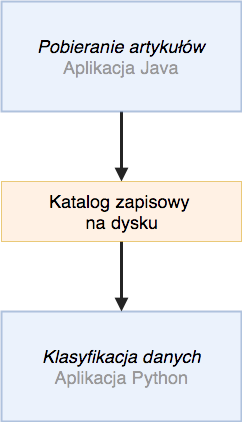
\includegraphics[width=0.25\linewidth]{img/architektura-pobierania}
	\caption{Architektura dostępu do danych}
	\label{fig:data-access}
\end{figure}

\section{Struktura dokumentów}

Zapisywane dokumenty domyślnie mają strukturę XMLową, co zapewnia uniwersalność i kompatybilność między użytymi narzędziami. 
\lstset{language=XML}
\begin{lstlisting}
<?xml version="1.0" encoding="UTF-8" standalone="yes"?>
<article>
    <author>Redakcja</author>
    <body>Egzekucja rozpoczęła się o godz. 20. [...]</body>
    <category>Historia</category>
    <keywords>narodowy dzień pamięci [...]</keywords>
    <source>http://www.focus.pl/artykul/1-m[...]</source>
    <title>1 marca - Narodowy Dzień [...]</title>
</article>
\end{lstlisting}
W niektórych przypadkach pobranie wszystkich danych było niemożliwe, dlatego mogą być one puste. Aplikacja, w fazie pobierania artykułów, odrzucała jednak te, które:
\begin{itemize}
\setlength\itemsep{0.6em}
\item nie posiadały tekstu,
\item nie posiadały kategorii,
\item nie posiadały źródła.
\end{itemize}
Zapisywane dokumenty przyjmowały nazwę z tytułu artykułu (w przypadku, gdy taki plik już istniał, był on nadpisywany); takie podejście pozwala na zbieranie artykułów fermentacyjnie, bez szkody dla aktualnie pobranych dokumentów. W przypadku, gdy tytuł artykułu był pusty, tworzony został skrót za pomocą funkcji haszującej \textit{MD5} \cite{md5-hash} z adresu źródła. Dzięki takiemu rozwiązaniu, katalog zawierał tylko unikalne artykuły pod względem treści. Pliki na dysku zapisywane były według źródła, z którego zostały pobrane; katalogi natomiast przyjmowały nazwy domen, tak jak zostało przedstawione na rysunku \ref{fetched-files-strucutre}. W celu łatwej manipulacji i zmiany ścieżek, w których są zapisywane dokumenty, zaproponowano interfejs o nazwie \textbf{PathResolver.class}, wymagający implementacji dwóch metod: \textbf{String resolveRelativePath(Article article)} oraz \textbf{String resolveFileName(Article article)}. 

\begin{lstlisting}[language=Java,basicstyle=\small, style=javaStyle]
public interface PathResolver {

	String resolveRelativePath(Article article);
	String resolveFileName(Article article);
    
}
\end{lstlisting}

Zmiana sposobu rozwiązywania ścieżek jest dokonywana poprzez zmianę implementacji w klasie \textbf{ArticleWriter.class}.

\begin{lstlisting}[language=Java,basicstyle=\small, style=javaStyle]
public interface ArticleWriter {

	void write(Article article) throws IOException;
	void setPathResolver(PathResolver strategy);

}
\end{lstlisting}



\begin{figure}[ht!]

\dirtree{%
.1 katalog docelowy .
.2 dobreprogramy.pl.
.3 \hyperref[dir1-file1]{''8475.txt''}.
.3 \hyperref[dir1-file2]{''8476.txt''}.
.2 historykon.pl.
.3 \hyperref[dir2-file1]{''3489.txt''}.
.3 \hyperref[dir2-file2]{''3490.txt''}.
.2 ...
}
\caption{Struktura plików pobranych dokumentów przez aplikację}
\label{fetched-files-strucutre}
\end{figure}

Nazwy wszystkich plików są unikalne względem katalogu, który został wyznaczony do zapisu. Mogą być bez przeszkód umieszczone w jednym katalogu, gdyby była taka potrzeba.
\section{Analiza zebranego korpusu}
Zebrany korpus składa się z ponad 22 tysięcy dokumentów i został zebrany z 9 różnych portali internetowych. Najlepszym źródłem wysokiej jakości dokumentów była Polska Agencja Prasowa, dlatego z tego portalu pobrano najwięcej dokumentów do analizy. Rozkład według portalu (wyjątkiem jest serwis PAP, ze względu na ilość danych) przedstawiony został na wykresie \ref{fig:rozklad-wg-zrodla}. 
\begin{figure}[hb!]
	\centering
	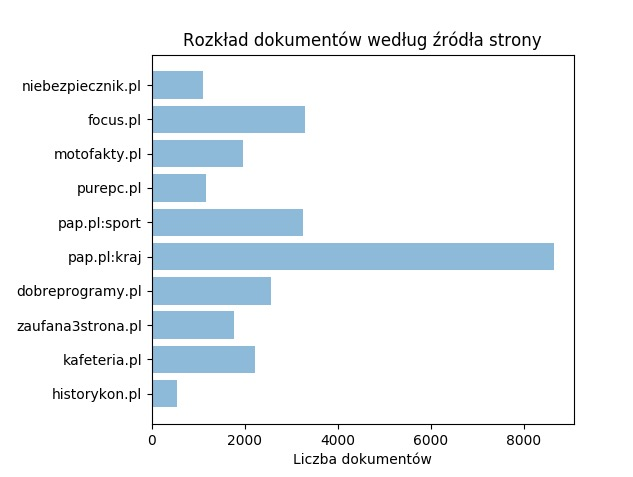
\includegraphics[width=0.8\linewidth]{img/articles-summary-by-source}
	\caption{Rozkład pobranych artykułów według źródła}
	\label{fig:rozklad-wg-zrodla}
\end{figure}
\begin{figure}[ht!]
	\centering
	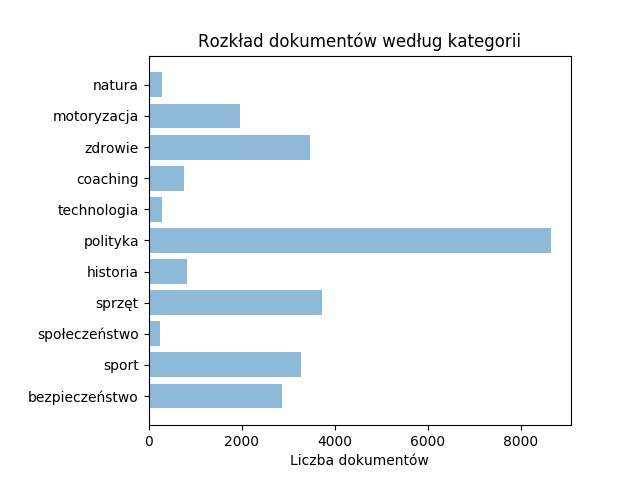
\includegraphics[width=0.8\linewidth]{img/articles-summary-by-category}
	\caption{Rozkład pobranych artykułów według kategorii}
	\label{fig:rozklad-wg-kategorii}
\end{figure}

\newpage

\subsection{Selekcja rozpatrywanych klas}
Na podstawie analizy rozkładu dokumentów na kategorie \ref{fig:rozklad-wg-kategorii} wyselekcjonowano 7 grup tematycznych które będą analizowane w pracy. \cite{deep-learning-methods-for-sub} Lista wybranych kategorii została zaprezentowana w tabeli \ref{tab:kategorie-z-artykulow}. Kategorie z liczbą artykułów poniżej 100 zostały odrzucone.
\begin{table}[ht!]
\centering
\caption{Rozłożenie liczby artykułów poszczególne kategorie}
\label{tab:kategorie-z-artykulow}
\begin{tabular}{|l|l|l|}
\hline
\textbf{kategoria} & \textbf{źródło}                                                                                        & \textbf{liczba dokumentów} \\ \hline
motoryzacja        & motofakty.pl                                                                                           & 1890                      \\ \hline
zdrowie            & \begin{tabular}[c]{@{}l@{}}kafeteria.pl\\ focus.pl/zdrowie\end{tabular}                                & 3823                      \\ \hline
polityka           & pap.pl/kraj                                                                                            & 8351                      \\ \hline
sport              & \begin{tabular}[c]{@{}l@{}}pap.pl/sport\\ focus.pl/sport\end{tabular}                                  & 2759                      \\ \hline
bezpieczeństwo     & \begin{tabular}[c]{@{}l@{}}zaufanatrzeciastrona.pl\\ dobreprogramy.pl\\ niebezpiecznik.pl\end{tabular} & 2311                      \\ \hline
sprzęt             & dobreprogramy.pl                                                                                       & 3942                      \\ \hline
historia             & historykon.pl                                                                                       & 1249                      \\ \hline
\end{tabular}
\end{table}


\subsection{Ograniczenie zbioru dokumentów}
Ograniczenie zbioru dokumentów polegało na odrzuceniu dokumentów, które posiadały mniej niż 200 znaków. Artykuły takie prawdopodobnie były reklamami, które mogłyby przeszkodzić w dalszej analizie. Następnie, do każdej kategorii wybierano 500 dokumentów, aby dane wejściowe dla każdej klasy były równe pod kątem ilościowym. Przetworzone pliki zapisane zostały do nowego katalogu z rozróżnieniem na kategorie, co zostało zaprezentowane na rysunku \ref{dir-by-categories}.

\begin{figure}[ht!]

\dirtree{%
.1 według\_kategorii .
.2 sport.
.3 \hyperref[dir1-file1]{''2475.txt''}.
.3 \hyperref[dir1-file2]{''2476.txt''}.
.2 polityka.
.3 \hyperref[dir2-file1]{''6489.txt''}.
.3 \hyperref[dir2-file2]{''6490.txt''}.
.2 ...
}
\caption{Struktura plików podzielona według klas}
\label{dir-by-categories}
\end{figure}

Tak skonstruowana struktura plików umożliwiała manipulację wbudowanymi narzędziami w bibliotece \textit{SciKit Learn}.


\section{Przetwarzanie wstępne}
W fazie wstępnego przetwarzania tekstu z pobranych plików w miarę możliwości usuwane są zbędne dane, takie jak adresy e-mail i cytaty. Forma tekstów jest ujednolicana, teksty zostają poddane lematyzacji i usunięciu słów nierelewantnych. Ogólny proces przepływ danych podczas przetwarzania wstępnego został pokazany na rysunku \ref{fig:process-flow}.

\begin{figure}[ht!]
	\centering
	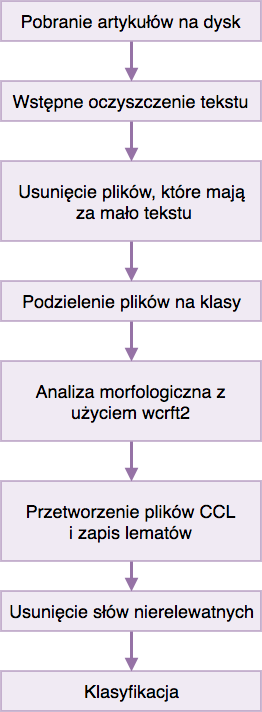
\includegraphics[width=0.3\linewidth]{img/process-flow}
	\caption{Schemat kolejnych kroków przetwarzania danych}
	\label{fig:process-flow}
\end{figure}

\clearpage
\subsection{Analiza morfologiczna tekstu}
Istotnym etapem przetwarzania tekstu było zastosowanie analizatora morfologicznego. W pracy wykorzystany został analizator morfologiczny Morfeusz 2 ze słownikiem SGJP, udostępniony w postaci REST API. Praca z serwisem odbywa się w sposób asynchroniczny, oznacza to, że najpierw należało przesłać plik tekstowy do analizatora, a następnie odpytywać serwer co jakiś czas, aby sprawdzić czy praca się zakończyła. Przykład użycia analizatora WCRFT2 przez REST API:

\lstdefinestyle{someShit}{
  numbers=left,
  stepnumber=0,
  numbersep=10pt,
  tabsize=3,
  showspaces=false,
  showstringspaces=false
}

\begin{itemize}
 \setlength\itemsep{2em}
\item Wysłanie pliku do serwera.
\begin{lstlisting}[style=pythonStyle]
# [POST] http://ws.clarin-pl.eu/nlprest2/base/upload
# Content-Type: 'binary/octet-stream'

def upload(file_path):
    with open(file_path, "rb") as file:
        file_bytes = file.read()
    req = urllib.request.Request(url + '/upload/', file_bytes, 
    {'Content-Type': 'binary/octet-stream'})
    return urllib.request.urlopen(req).read().decode("utf-8")

\end{lstlisting}
Serwer w odpowiedzi wyśle ID zapisanego pliku (id\_pliku).

\item Rozpoczęcie przetwarzania tekstu z użyciem analizatora WCRFT2.
\begin{lstlisting}[style=pythonStyle]
# [POST] http://ws.clarin-pl.eu/nlprest2/base/startTask
# data = { 
#	'lpmn': 'any2txt|wcrft2, 
#	'user': '209897@student.pwr.edu.pl', 
#	'file': id_pliku 
# }

def process(data):
    json_data = json.dumps(data).encode('utf-8')
    start_task_req = urllib.request.Request(url=url + '/startTask/')
    start_task_req.add_header('Content-Type', 'application/json')
    start_task_req.add_header('Content-Length', len(json_data))
    task_id = urllib.request
        .urlopen(start_task_req, json_data)
        .read()
        .decode("utf-8")
    time.sleep(0.1)
    
\end{lstlisting}
Serwer w odpowiedzi wyśle ID rozpoczętego zadania (id\_zadania).

\item Sprawdzenie czy analiza się zakończyła.
\begin{lstlisting}[style=pythonStyle]
# [GET] http://ws.clarin-pl.eu/nlprest2/base/getStatus/{id_zadania}   
    reqUrl = url + '/getStatus/' + task_id
    get_status_req = urllib.request.Request(reqUrl)
    status_response = urllib.request.urlopen(get_status_req)
    data = json.load(status_response)
    while data["status"] == "QUEUE" or data["status"] == "PROCESSING":
        time.sleep(0.1)
        get_status_req = urllib.request.Request(reqUrl)
        status_response = urllib.request.urlopen(get_status_req)
        data = json.load(status_response)
    if data["status"] == "ERROR":
        print("Error " + data["value"])
        return None
    return data["value"]
\end{lstlisting}
Serwer w odpowiedzi poinformuje o błędzie ("\textit{ERROR}"), przetwarzaniu ("\textit{PROCESSING}") lub oczekiwaniu na przetworzenie ("\textit{QUEUE}").

\item Pobranie pliku wynikowego.
\begin{lstlisting}[style=pythonStyle]
# [GET] http://ws.clarin-pl.eu/nlprest2/base/download/{id_pliku}
def process_file(source_file, output_file):
    file_id = upload(source_file)
    print("[F] Processing: " + source_file)
    data = {'lpmn': lpmn, 'user': user, 'file': file_id}
    data = process(data)
    data = data[0]["fileID"]
    download_req = urllib.request.Request(url + '/download' + data)
    content = urllib.request
        .urlopen(download_req)
        .read()
        .decode("utf-8")

    output_file = output_file + ".ccl.xml"
    save_text(output_file, content)
\end{lstlisting}
\end{itemize}

W projekcie wzorowano się na udostępnionym kodzie dla języka Python 2.6 \cite{wcrf-api-reference}, który został odpowiednio dostosowany do nowszej wersji języka.



\subsection{Ustalenie podstawowej postaci wyrazów}
Formy podstawowe wyrazów (haseł) zostały ustalone dzięki analizatorowi WCRFT2, który zwracał XML (CCL) jako plik wynikowy. \cite{cclFormat}

\lstset{language=XML}
\begin{lstlisting}
<?xml version="1.0" encoding="UTF-8"?>
<!DOCTYPE chunkList SYSTEM "ccl.dtd">
<chunkList>
 <chunk id="ch1" type="p">
  <sentence id="s1">
   <tok>
    <orth>Niemalże</orth>
    <lex disamb="1">
    	<base>niemalże</base><ctag>qub</ctag>
    </lex>
   </tok>
   <tok>
    <orth>od</orth>
    <lex disamb="1">
    	<base>od</base><ctag>prep:gen:nwok</ctag>
    </lex>
   </tok>
   <tok>
    <orth>początku</orth>
    <lex disamb="1">
    	<base>początek</base><ctag>subst:sg:gen:m3</ctag>
   </lex>
   </tok>
   </sentence>
   </chunk>
</chunkList>
\end{lstlisting}

 Do odczytania pliku wykorzystano domyślny parser w języku Python o nazwie \textit{ElementTree}. Napisana funkcja \textit{ccl\_to\_lemma} przyjmowała plik w formacie XML (CCL) oraz zapisywała plik tekstowy z oddzielonymi przecinkami formami podstawowymi.
 

 
\begin{lstlisting}[style=pythonStyle]
def ccl_to_lemma(input_file, output_file):
    tree = ElementTree.parse(input_file)
    root = tree.getroot()
    base_words = []
    for token in root.getiterator('tok'):
        base = token.find('lex').find('base').text
        base_words.append(base)

    output_file = output_file + ".lemma"
    content = " ".join(base_words)
    save_text(output_file, content)
\end{lstlisting}



Z uwagi na wykorzystanie gotowego analizatora morfologicznego, w pracy przyjęto zbiór tagów gramatycznych autorstwa Adama Przepiórkowskiego \cite{polishGrammarTagset}, zaprezentowanych w tabeli \ref{klasy-gramatyczne}, który jest wykorzystywany przez ten analizator. Pełny spis klas można znaleźć na stronie \url{http://nkjp.pl/poliqarp/help/ense2.html}.
\begin{table}[ht!]
\centering
\caption{Klasy gramatyczne}
\label{klasy-gramatyczne}
\begin{tabular}{|l|l|}
\hline
\textbf{fleksem}         & \textbf{skrót} \\ \hline
rzeczownik               & subst          \\ \hline
rzeczownik deprecjatywny & depr           \\ \hline
liczebnik główny         & num            \\ \hline
liczebnik zbiorowy       & numcol         \\ \hline
przymiotnik              & adj            \\ \hline
przymiotnik przyprzym.   & adja           \\ \hline
przymiotnik poprzyimkowy & adjp           \\ \hline
przymiotnik predykatywny & adjc           \\ \hline
przysłówek               & adv            \\ \hline
zaimek nietrzecioosobowy & ppron12        \\ \hline
zaimek trzecioosobowy    & ppron3         \\ \hline
zaimek siebie            & siebie         \\ \hline
forma nieprzeszła        & fin            \\ \hline
forma przyszła być       & bedzie         \\ \hline
aglutynant być           & aglt           \\ \hline
pseudoimiesłów           & praet          \\ \hline
rozkaźnik                & impt           \\ \hline
bezosobnik               & imps           \\ \hline
bezokolicznik            & inf            \\ \hline
im. przys. współczesny   & pcon           \\ \hline
im. przys. uprzedni      & pant           \\ \hline
odsłownik                & ger            \\ \hline
im. przym. czynny        & pact           \\ \hline
im. przym. bierny        & ppas           \\ \hline
winien                   & winien         \\ \hline
predykatyw               & pred           \\ \hline
przyimek                 & prep           \\ \hline
spójnik współrzędny      & conj           \\ \hline
spójnik podrzędny        & comp           \\ \hline
kublik                   & qub            \\ \hline
skrót                    & brev           \\ \hline
burkinostka              & burk           \\ \hline
wykrzyknik               & interj         \\ \hline
interpunkcja             & interp         \\ \hline
ciało obce               & xxx            \\ \hline
forma nierozpoznana      & ign            \\ \hline
\end{tabular}
\end{table}

\clearpage
\subsection{Analiza słów nierozpoznanych}

Po przeprowadzeniu analizy morfologicznej dokonano analizy klas gramatycznych w obu korpusach \ref{fig:corpus-ign}. Na przedstawionych rysunkach widać, że dużą część korpusu stanowią wyrazy, które nie zostały rozpoznane przez analizator WCRFT2 (klasa \textit{ign})
\begin{figure}[ht!]
	\centering
	\subfloat[Artykuły]{{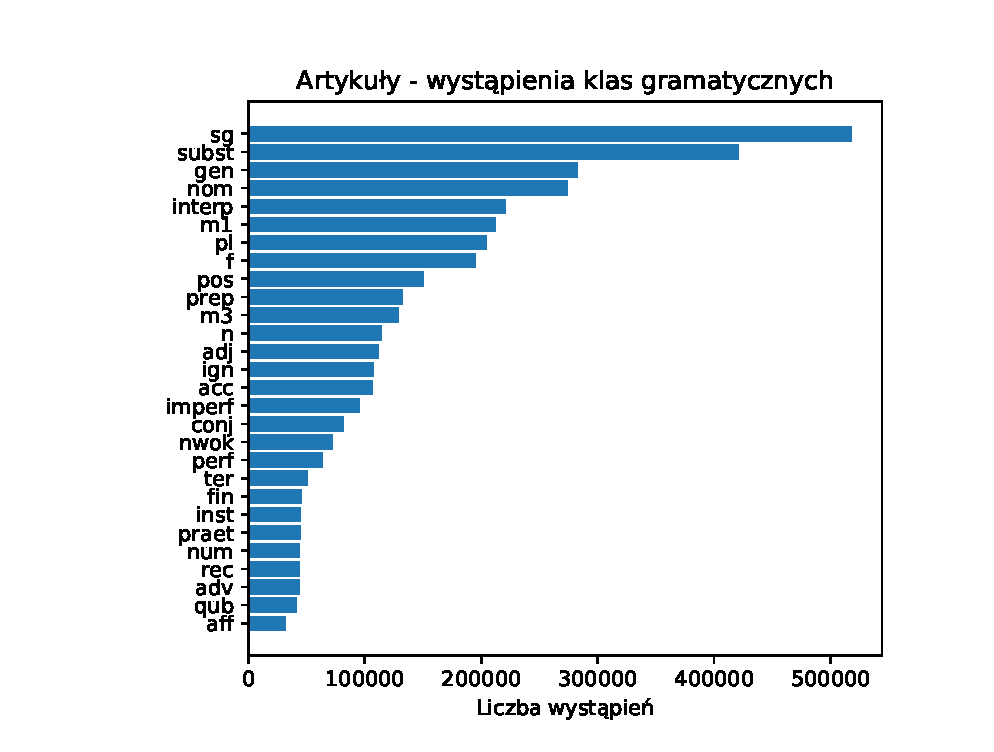
\includegraphics[width=0.8\linewidth]{img/gram-classes-articles}}}
    \qquad
    \subfloat[Wikipedia]{{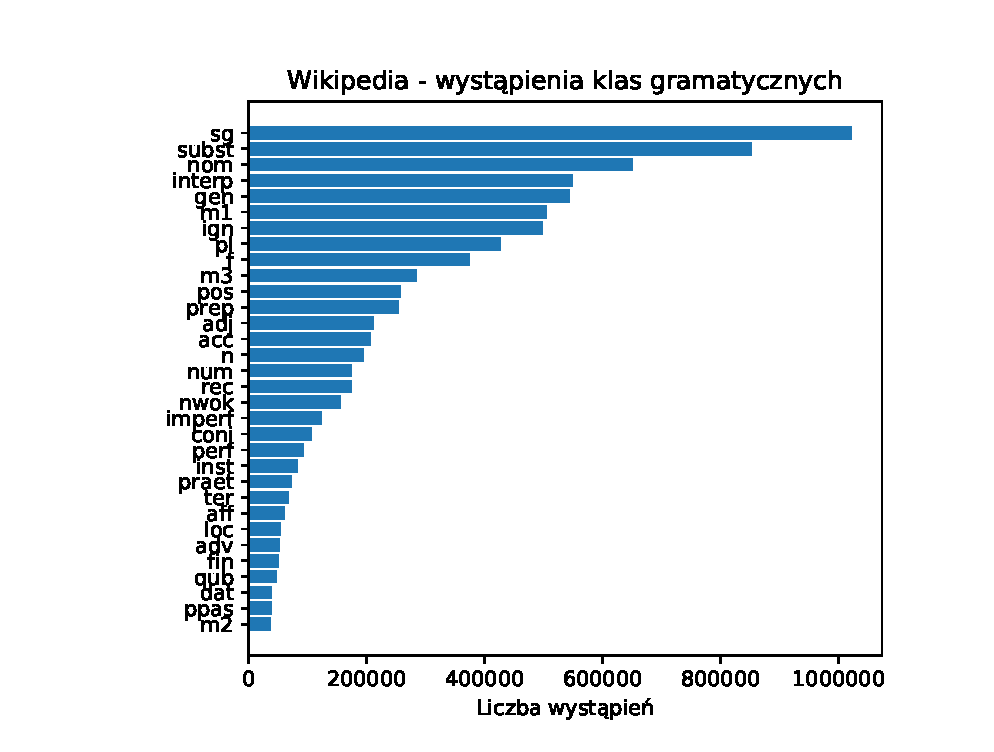
\includegraphics[width=0.8\linewidth]{img/gram-classes-wikipedia}}}
	\caption{Porównanie wystąpień klas gramatycznych w obu korpusach}
    \label{fig:corpus-ign}
\end{figure}

W przypadku korpusu \textit{Artykuły} nie rozpoznano około 5.19\% wyrazów w stosunku do całego korpusu. W korpusie \textit{Wikipedia} wartość ta wynosi tylko 1.12\%. Rozbieżności między tymi wartościami wynikają najprawdopodobniej z literówek, jakie mogły zaistnieć podczas pisania artykułów. W artykułach z platformy Wikipedia często są one poprawiane i redagowane przez więcej niż jedną osobę. 
W pełni automatyczna poprawa tekstu byłaby zadaniem trudnym; takie działanie mogłoby skutkować pogorszeniem wyników, jeśli słowo zostałoby nieprawidłowo zinterpretowane. W celu poprawy jakości zebranych danych, wyznaczone zostały najczęściej występujące nierozpoznane słowa zaprezentowane na rysunku \ref{fig:freq-ign-words}.

\begin{figure}[ht!]
	\centering
	\subfloat[Artykuły]{{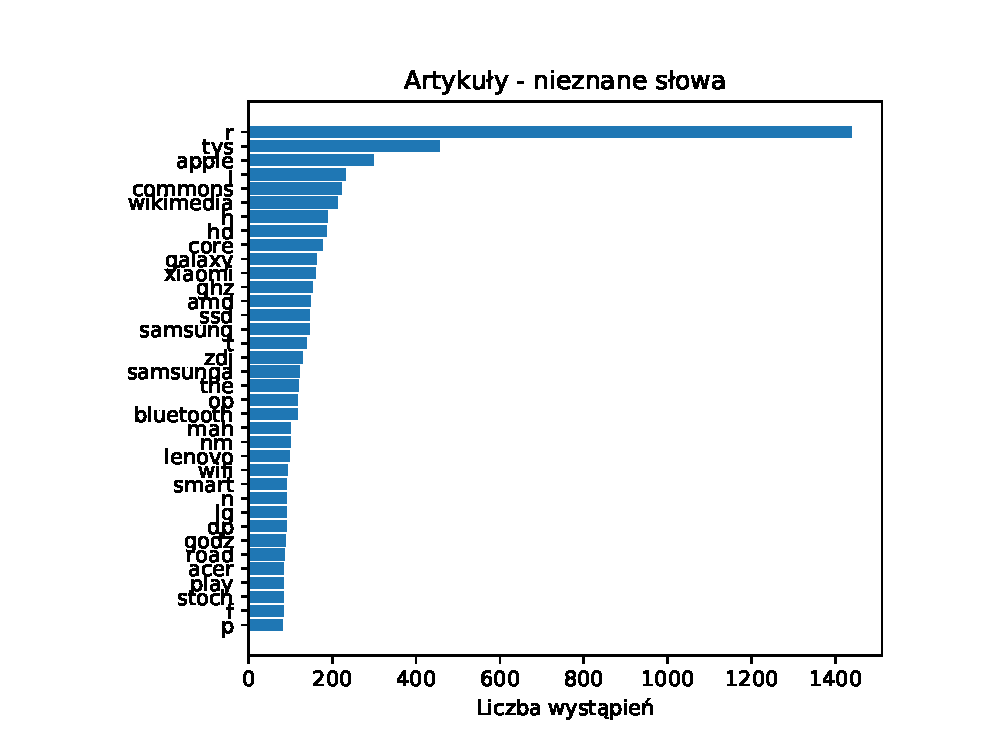
\includegraphics[width=0.8\linewidth]{img/unknown-words-articles}}}
    \qquad
    \subfloat[Wikipedia]{{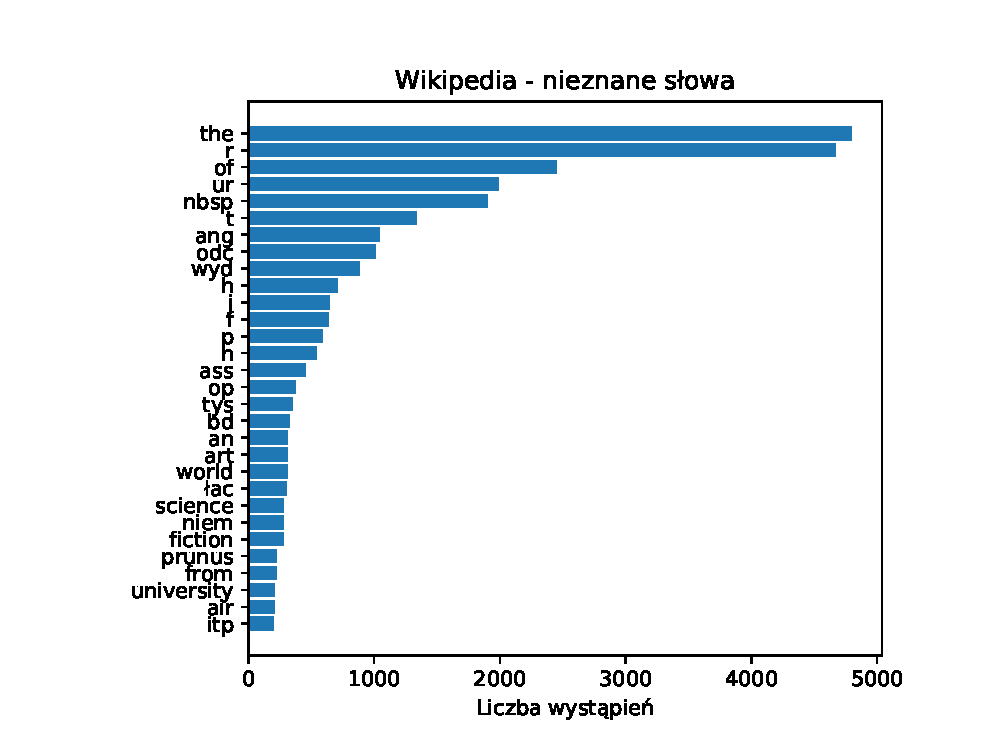
\includegraphics[width=0.8\linewidth]{img/unknown-words-wikipedia}}}
	\caption{Porównanie wystąpień nierozpoznanych form w obu korpusach}
    \label{fig:freq-ign-words}
\end{figure}

Formami nierozpoznanymi okazały się w głównej mierze nazwy własne. W obu korpusach są one częścią istotnych cech, które sugerują daną grupę tematyczną, dlatego pozostały w korpusach bez zmian. \textit{r} - prawdopodobnie jest to pozostałość po podziale wartości liczbowej roku oraz skrótu \textit{r.}.
Usunięto jedynie kilka wyrazów
\begin{itemize}
\item \textit{nbsp} (ang. non breaking space) - kod HTML dla spacji niełamliwej używanej w kodzie \cite{nbsp-wikipedia}
\item \textit{commons} oraz \textit{wikipedia} - od nazwy własnej Wikipedia Commons, prawdopodobnie błąd podczas pobierania
\end{itemize}

Należy jednak pamiętać, że klasyfikowane artykuły zawsze zawierać będą pewien odsetek tekstów, które są błędnie napisane. Dlatego zdecydowano się na usunięcie jedynie oczywistych błędów popełnionych podczas implementacji programów zbierających korpusy.

\subsection{Usunięcie wyrazów nierelewantnych}
Podczas analizy tekstu istotnym aspektem jest jakość analizowanych danych i dokumentów. W pracach dotyczących klasyfikacji tematycznej częstą praktyką jest usuwanie słów nierelewantnych w fazie przetwarzania  \cite{introInfoRetrieval}\cite{indeksowanietresci}\cite{mykowiecka}. Do słów nierelewantnych zalicza się wyrazy, które najczęściej występują w danym języku (ang. stop words). Dzięki temu współczynnikowi, jakość klasyfikacji ulega poprawie poprzez pomijanie mało istotnych wyrazów. Dodatkową zaletą jest mniejsze zapotrzebowanie na pamięć oraz moc obliczeniową, ponieważ przetwarzanych danych jest mniej. W pracy wykorzystano listę wyrazów, która została udostępniona na stronie \textit{https://www.ranks.nl/stopwords/polish} \cite{polishStopwords} w postaci tabeli.

\subsection{Analiza zawartości korpusu}
Kluczowym etapem okazała się ręczna analiza zawartości korpusu z wykorzystaniem takich metod jak modelowanie tematów (ang. topic modeling). Modelowanie tematów jest techniką analizy dużych zbiorów dokumentów; modele automatycznie wyszukują tematy w tekście z wykorzystaniem ukrytych zmiennych losowych. Technika ta często jest wykorzystywana do rekomendacji tagów, wyszukiwania słów kluczowych, kategoryzacji tekstów. \cite{about-lda} W pracy wykorzystano gotową implementację \textit{LDA} (Latent Allocation Dirichlet) z biblioteki \textit{SciKitLearn} w celu analizy zawartości zebranego korpusu. Wyniki analizy \ref{tab:lda-result} wykazały, że zawartość korpusu, mimo starannych prób usunięcia wszystkich wyrazów mogących powodować błędne wyniki, nie była idealna.



\begin{table}[ht!]
\centering
\caption{Wynik modelowania tematycznego przy pomocy LDA}
\label{tab:lda-result}
\begin{tabular}{|l|l|}
\hline
\multicolumn{1}{|c|}{Topic 0} & mecz rok polska 00 minuta pap pierwsza druga miejsce raz                       \\ \hline
Topic 1                       & urządzenie model smartfon móc sprzęt nowa ekran producent można wersja         \\ \hline
Topic 2                       & skóra kobieta móc należeć choroba woda często czas zabieg można                \\ \hline
Topic 3                       & samochód pojazd prezydent kierowca powiedzieć zostać ustawa złoty projekt auto \\ \hline
Topic 4                       & metr pkt polska konkurs niemcy pap stefan rok miejsce już pozycja seria        \\ \hline
Topic 5                       & niebezpiecznik dana serwer firma atak serwis móc sieć informacja błąd          \\ \hline
Topic 6                       & rok polski polska lato czas były państwo pap była wojna więc                   \\ \hline
\end{tabular}
\end{table}

W zawartości korpusu znalazły się słowa, które mogły dać klasyfikatorom jednoznaczne podpowiedzi, do której grupy przynależy tekst, na przykład \textit{pap} oraz \textit{niebezpiecznik}. W celu usunięcia niechcianych wyrazów dodano je do listy słów nierelewantnych. Analiza była przeprowadzana tak długo, dopóki wszystkie niechciane słowa nie zostały usunięte z wyników pracy \textit{LDA}. Ostatecznie zliczono wszystkie formy podstawowe wyrazów dla każdej kategorii i przedstawiono je na rysunku \ref{fig:rozklad-lemmatow-wg-zrodla}.

\begin{figure}[ht!]
	\centering
	\subfloat[Artykuły]{{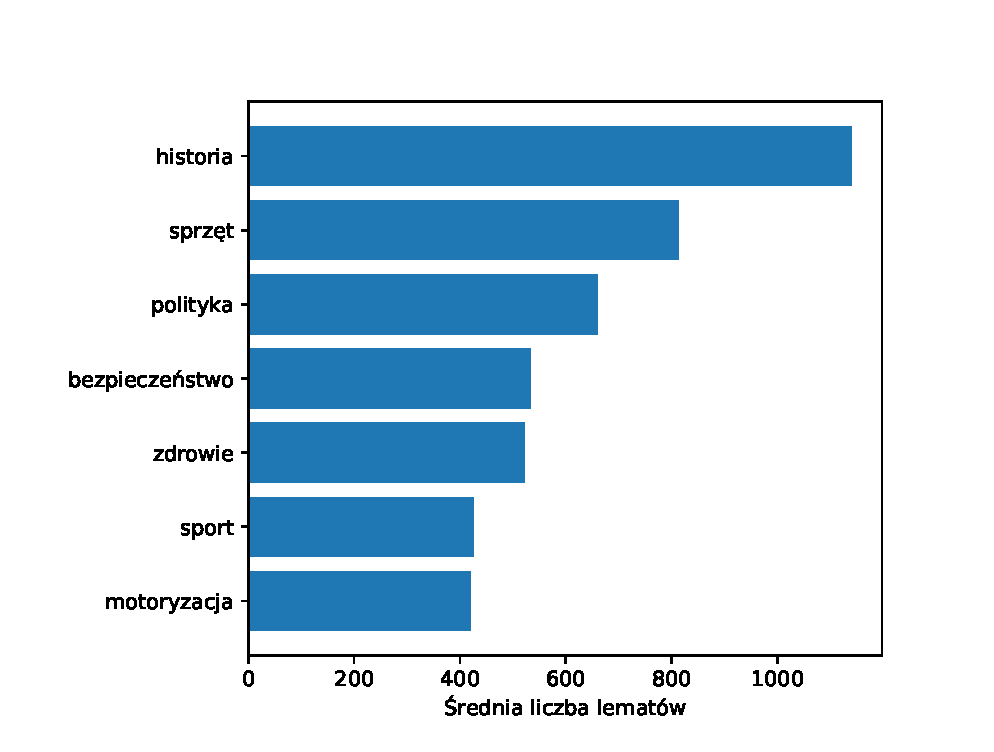
\includegraphics[width=0.8\linewidth]{img/avg-lemma-count-articles}}}
    \qquad
    \subfloat[Wikipedia]{{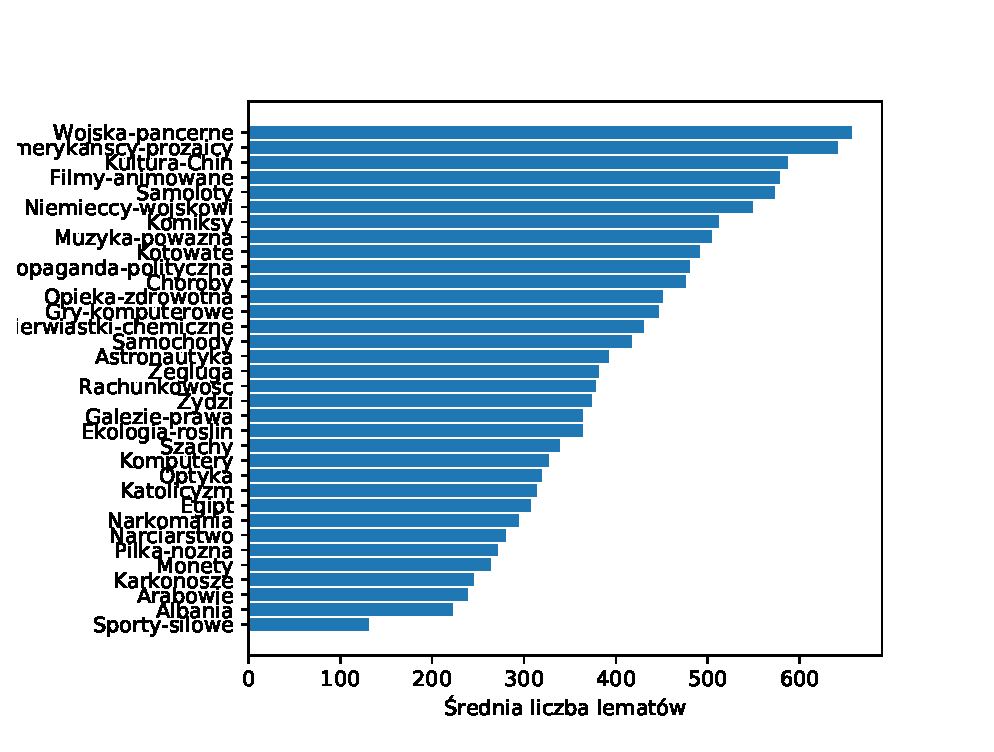
\includegraphics[width=0.8\linewidth]{img/avg-lemma-count-wikipedia}}}
	\caption{Rozkład średniej liczby lematów według kategorii}
   \label{fig:rozklad-lemmatow-wg-zrodla}
\end{figure}
\newpage
\section{Metody klasyfikacji tekstu}
W pracy zdecydowano się na przetestowanie dwóch różnych metod klasyfikacji, \textit{Bag-Of-Words} oraz \textit{fastText}, który jest pochodną \textit{word2vec}.
\subsection{Bag-Of-Words}
Aby móc poddać tekst klasyfikacji, konieczne jest wstępne przetworzenie tekstu wejściowego i przedstawienie go w postaci macierzy lub, w przypadku prostszych metod, wektora wierszowego dla danego tekstu. Istnieje wiele różnych sposobów wektoryzacji dokumentów; najprostszym i najczęściej stosowanym \cite{BoulisText} jest model \textit{Bag-Of-Words}. Każdy dokument jest przedstawiany w postaci wektora wierszowego, który zawiera liczbę wystąpień słowa w danym dokumencie.\cite{joulin2016bag}
\subsubsection*{Przykład Bag-of-Words}
Utworzenie \textit{Bag-of-Words} na przykładzie dwóch dokumentów \cite{bow-example} wyglądałoby następująco: \\ \hfill
\begin{lstlisting}[style=someShit]
dokument 1: "The Sun is a star. Sun is beautiful."
dokument 2: "The Moon is a satellite."
\end{lstlisting}
Na podstawie zadanych dwóch dokumentów utworzony zostanie słownik z unikalnymi słowami. Liczba wszystkich unikalnych słów będzie również liczbą kolumn w każdym wektorze wierszowym dla całego korpusu dokumentów.\\

Przykładowe dokumenty składają się z 8 unikalnych słów, dlatego każdy dokument jest reprezentowany jako 8-elementowy wektor wierszowy i został przedstawiony na rysunku \ref{vectors-bow}.

\begin{table}[ht!]
\centering
\caption{Tabela wektorów Bag-Of-Words}
\label{vectors-bow}
\begin{tabular}{|l|c|c|}
\hline
\multicolumn{1}{|c|}{\textbf{słowo}} & \textbf{dokument 1} & \multicolumn{1}{l|}{\textbf{dokument 2}} \\ \hline
The                                                          & 1                   & 1                                                                \\ \hline
Sun                                                          & 2                   & 0                                                                \\ \hline
is                                                           & 2                   & 1                                                                \\ \hline
a                                                            & 1                   & 1                                                                \\ \hline
star                                                         & 1                   & 0                                                                \\ \hline
beautiful                                                    & 1                   & 0                                                                \\ \hline
Moon                                                         & 0                   & 1                                                                \\ \hline
satellite                                                    & 0                   & 1                                                                \\ \hline
\end{tabular}
\end{table}

Cyfra pierwsza '1' w obu dokumentach oznacz, że w dokumencie tylko raz wystąpiło słowo 'The'. Druga cyfra ('2') w dokumencie pierwszym oznacza, że słowo 'Sun' wystąpiło dwa razy, natomiast w dokumencie drugim ('0') ani razu nie pojawiło się słowo 'Sun'.
\begin{lstlisting}[caption=Utworzone wektory, style=someShit]
dokument 1: [1, 2, 2, 1, 1, 1, 0, 0]
dokument 2:  [1, 0, 1, 1, 0, 0, 1, 1]
\end{lstlisting}
\subsubsection*{Ustalenie wag - \textit{tf-idf}}
Algorytm \textit{tf-idf} służy do określania wag słów względem całego korpusu. Jeśli słowo pojawia się często we wszystkich dokumentach, jego znaczenie maleje, ponieważ prawdopodobnie nie wnosi ono żadnej praktycznej wiedzy. \textit{tf-idf} mierzy znaczenie, a nie częstotliwość i jego wartość jest obliczana według wzoru\cite{tfidf-eq}:

\begin{equation}
Wt,d = TFt,d log(N/DFt)
\end{equation}

Gdzie:
\begin{itemize}
\item $TFt,d$ - oznacza liczbę wystąpień słów $t$ w dokumentach $d$,
\item $DFt$ - oznacza liczbę dokumentów zawierających słowo $t$,
\item $N$ - oznacza liczbę wszystkich dokumentów w korpusie.
\end{itemize}

\subsubsection*{Implementacja Bag-Of-Words}
W pracy użyto narzędzia o nazwie \textit{CountVectorizer} z biblioteki \textit{SciKit Learn}, która służy do wyodrębniania cech numerycznych z treści tekstowej, a mianowicie\cite{skl-reference}:
\begin{itemize}
\setlength\itemsep{0.6em}
\item tokenizuje ciągi znaków, 
\item zlicza wystąpienia tokenów w każdym dokumencie,
\item usuwa \textit{stop words} z zadanej listy,
\item normalizuje i ustala wagi, liczbę próbek / liczbę dokumentów.
\end{itemize}

Tekstem wejściowym dla zastosowanego narzędzia \textit{CountVectorizer} były zlematyzowane teksty (hasła) uzyskane w fazie przetwarzania wstępnego. Kapitalizacja wszystkich wyrazów została usunięta i wszystkie litery zostały zamienione na małe. Efektem działania \textit{CountVectorizera} jest macierz terminów \textit{dokument} (ang. document-term), która opisuje częstotliwość występowania tokenów w zbiorze dokumentów. Kolumny odpowiadają kolejnym wyrazom, a wiersze dokumentom, tak jak przedstawiono w tabeli \ref{countvectorizer-output}.

\begin{table}[ht!]
\centering
\caption{Macierz dokument-wyrażenie}
\label{countvectorizer-output}
\begin{tabular}{|c|c|c|c|c|c|c|c|c|}
\hline
   & The & Sun & is & a & star & beautiful & Moon & satellite \\ \hline
D1 & 1   & 2   & 2  & 1 & 1    & 1         & 0    & 0         \\ \hline
D2 & 1   & 0   & 1  & 1 & 0    & 0         & 1    & 1         \\ \hline
\end{tabular}
\end{table}
\newpage
Końcową optymalizacją jest zastosowanie normalizacji \textit{tf-idf} w celu ustalenia wag lematów w macierzy. Tak przygotowana macierz może już być wprowadzona do klasyfikatora w celu nauki oraz późniejszych testów. Implementacja została zaprezentowana na listingu poniżej.

\begin{lstlisting}[style=pythonStyle]
#funkcja uruchamiajaca test BagOfWords
def invoke(
      data_train, data_test, #dane uczace
      target_train, target_test, #dane testowe
      clf, iterations): #klasyfikator, ilosc iteracji
    
    	#zmienne tymczasowe do wyznaczenia wartosci srednich
    fit_time_acc = 0 
    predict_time_acc = 0
    accuracy_acc = 0
    f1_acc = 0

	#petla iteracyjna
    for iter_index in range(0, iterations):
    	#wykonanie obliczen dla jednego kroku
        predicted, fit_time, predict_time = iter_step(
        	data_train, data_test, target_train, clf)
            
        #sumowanie obliocznych wynikow
        fit_time_acc += fit_time
        predict_time_acc += predict_time
        accuracy_acc += accuracy_score(target_test, predicted)
        f1_acc += f1_score(target_test, predicted, average='micro')

	#wyznaczenie wartosci srednich
    mean_fit_time = fit_time_acc / iterations
    mean_predict_time = predict_time_acc / iterations
    mean_accuracy = accuracy_acc / iterations
    mean_f1_acc = f1_acc / iterations

	#zwrocenie wynikow
    return mean_f1_acc, mean_accuracy, mean_fit_time, mean_predict_time


def iter_step(data_train, data_test, target_train, classifier):
	#pobranie listy slow nierelewatnych
    stop_words_list = read_stop_words_list("../data/stop_words/list.txt")
    countVectorizer = CountVectorizer(stop_words=stop_words_list)
    tfidf_vectorizer = TfidfVectorizer()
    
    	#stworzenie procesu
    pipeline = Pipeline([
    	('cnt', countVectorizer),
        ('vect', tfidf_vectorizer),
        ('clf', classifier)])

	#nauczenie wszystkich elementów w 'pipeline'
    start = time.time()
    pipeline = pipeline.fit(data_train, target_train)
    end = time.time()
    	#wyznaczenie czasu nauki
    fit_time = (end - start)

	#klasyfikacja danych testowych
    start = time.time()
    predicted = pipeline.predict(data_test)
    end = time.time()
    	#wyznaczenie czasu predykcji
    predict_time = (end - start)

	#zwrocenie wyników
    return predicted, fit_time, predict_time

\end{lstlisting}

\subsubsection{Badane klasyfikatory}
W pracy zdecydowano się na wykorzystanie trzech klasyfikatorów; do tego celu wybrano 3 najczęściej wykorzystywane klasyfikatory w pracach dotyczących klasyfikacji tematycznej. \cite{walkowiak2018} \cite{text-classification-stanford}\cite{maciej-baj}
\begin{itemize}
 \setlength\itemsep{2em}
\item \textbf{Wielomianowy naiwny klasyfikator bayesowski} (ang. Multinomial Naive Bayes) - metoda, która określa przynależność danego obiektu do klasy na podstawie prawdopodobieństwa. \cite{internet-stat-book} Klasyfikacja odbywa się przy wykorzystaniu cech z wartościami dyskretnymi (np. liczba słów dla klasyfikacji tekstu). Rozkład wielomianowy zwykle wymaga liczby elementów całkowitych. Jednak w praktyce mogą być to również liczby ułamkowe, występujące w przypadku wektoryzacji \textit{TF-IDF}. \cite{skl-reference}

\item \textbf{Liniowa maszyna wektorów nośnych} (ang. Linear Support Vector Machine) - SVM to zestaw nadzorowanych metod uczenia używanych do klasyfikacji. Metoda polega na wyznaczaniu granic hiperpłaszczyzny oddzielającej próbki każdej klasy. W pracy wykorzystano SVM z liniową funkcją separującą; oznacza to, że przestrzenie są tak dzielone, aby odległość pomiędzy każdym jej punktem, a najbliższym punktem innej płaszczyzny był jak największy. \cite{internet-stat-book}

\item \textbf{Drzewo decyzyjne} (ang. Decision Tree) - to nadzorowana metoda uczenia stosowana do klasyfikacji i regresji. Tworzony jest model, który jest w stanie klasyfikować dane poprzez naukę prostych reguł decyzyjnych wywnioskowanych z danych uczących. Im głębsze drzewo, tym bardziej złożone reguły decyzyjne. \cite{skl-reference}
\end{itemize}

\subsection{fastText}
\textit{fastText} to metoda klasyfikacji, stworzona w laboratorium AI Research (FAIR) w Facebooku jako projekt open-source, aby sprostać potrzebie zrozumienia znaczenia dużych zbiorów tekstów. Biblioteka została zaprojektowaną tak, aby ułatwić tworzenie skalowalnych rozwiązań do reprezentacji i klasyfikacji tekstu. Jest to stosunkowo nowa metoda wykorzystywana do kategoryzacji tekstu. W założeniu twórców ma ona umożliwiać klasyfikację bardzo dużych ilości danych w krótkim czasie przy niskich wymaganiach sprzętowych. Według autorów, \textit{fastText} potrafi klasyfikować 500 tysięcy zdań na 300 tysięcy kategorii w mniej niż 5 minut na zwykłych komputerach domowych. \cite{faster-better-fasttext}

\textit{FastText} wykorzystuje technikę osadzonych słów (ang. word embedding) i domyślnie używa klasyfikatora Softmax \cite{walkowiak2018}. Wykorzystuje także tablicę przeglądową (ang. lookup table) z haszowaniem dla n-gramów, składających się ze słów lub znaków. Każdy dokument reprezentowany jest jako średnia z osadzania słów. Zaletą tej metody jest zdolność do tworzenia wektorów dla dowolnych słów, nawet tych, które są niepoprawnie napisane (ponieważ w rzeczywistości wektory te zbudowane są z podłańcuchów znaków w nim zawartych). Dzięki temu, wektory mogą być budowane na podstawie złączonych ze sobą tylko dwóch słów. Istotną zaletą jest również zdecydowanie krótszy czas klasyfikacji oraz nauki w porównaniu do innych metod. Jest to rozszerzenie metody \textit{word2vec}, w której każde słowo w korpusie jest traktowane jako atomowa jednostka i generowany jest dla niej oddzielny wektor. \cite{joulin2016bag}  \textit{fastText} domyślnie ignoruje kolejność słów, podobnie jak metoda \textit{BoW}. Aby uwzględnić lokalną kolejność słów, \textit{fastText} pozwala na użycie n-gramów, jednak funkcja ta ostatecznie nie była używana w eksperymentach.\cite{joulin2016fasttext}



\subsubsection{Działanie word2vec}
Modele \textit{word2vec} oraz \textit{fastText} zostały stworzone przez zespół prowadzony przez Tomasa Mikolova z Google. Algorytm przyjmuje duży korpus tekstu jako wejście i tworzy przestrzeń wektorową, \cite{nlp-from-scratch} zazwyczaj o kilkuset wymiarach z każdym unikalnym wyrazem w korpusie, któremu przypisuje odpowiedni wektor w przestrzeni. Wektory słów są umieszczane w przestrzeni wektorowej w taki sposób, że słowa, które mają wspólne konteksty w korpusie, znajdują się blisko siebie w przestrzeni. Przykład takich relacji został zaprezentowany na rysunku \ref{fig:word2vec-relation}. \cite{word2vec-google}

\begin{figure}[ht!]
	\centering
	\fbox{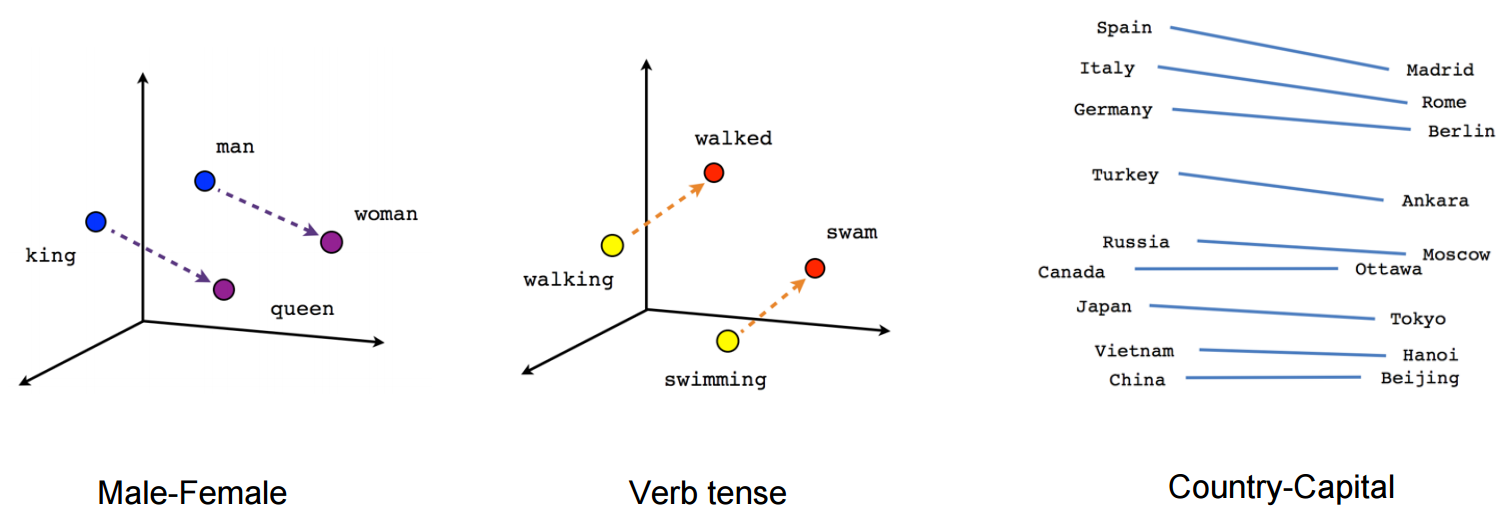
\includegraphics[width=1\linewidth]{img/linear-relationships}}
	\caption{Liniowa zależność word2vec}
	\label{fig:word2vec-relation}
\end{figure}

\subsubsection{Implementacja Python}
Biblioteka \textit{fastText} została oryginalnie napisana w języku C++ i nie ma dostępnych żadnych oficjalnych \textit{wrapperów} do języka Python. Jednak w sieci istnieje wiele rozwiązań, które pozwalają na wykorzystanie \textit{fastText} w języku Python. W pracy wykorzystano wrapper o nazwie \textit{ShallowLearn} (więcej informacji \url{https://github.com/giacbrd/ShallowLearn}), który jest zbiorem modeli uczenia opartym na płytkich podejściach do sieci neuronowych (np. \textit{word2vec} i \textit{fastText}). Do wykorzystanego wrappera należało również stworzyć odpowiedni adapter, który realizował funkcję konwertera danych wejściowych do oczekiwanego przez wrapper format. Dodatkowo otrzymywane przez \textit{ShallowLearn} wyniki musiały zostać poddane odpowiedniemu przetworzeniu tak, aby dane wyjściowe były reprezentowane w takiej samej postaci, jak ma to miejsce w przypadku implementacji \textit{Bag-Of-Words}. W tym celu stworzona została klasa \textit{calc\_adaper.py}, która poprawiała kompatybilność z biblioteką \textit{SciKit-Learn}. Możliwe stało się wykorzystanie metod dostarczanych przez interfejs biblioteki, \textit{fit} oraz \textit{predict}.